\documentclass{poly}
\usepackage{main}

\title{Suites arithmétiques}
\date{}
\author{TSTMG1}

\begin{document}
\maketitle
\section{Termes d'une suite arithmétique}
\begin{definition}[Rappel]
Une suite arithmétique est une suite numérique $\left(u_n\right)_{n \in \N}$ définie par son \textbf{premier terme} $u_0$ et un nombre $r$ appelé la \textbf{raison}, tel que chaque terme $u_n$ pour $n > 0$ est obtenu en ajoutant $r$ au terme précédent :
\begin{equation*}
u_n = u_{n-1} + r
\end{equation*} 
\end{definition}
\begin{example}
\begin{itemize}
\item La suite
\begin{equation*}
0; 2; 4; 6; 8; 10; \dots
\end{equation*}
est la suite de premier terme $0$ et de raison $2$.
\begin{center}
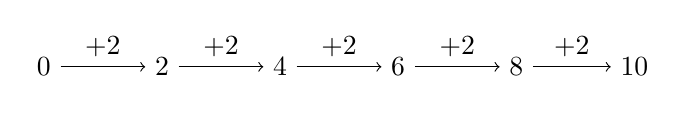
\begin{tikzpicture}
\node (A) at (0,0) {$0$};
\node (B) at (1.5,0) {$2$};
\node (C) at (3,0) {$4$};
\node (D) at (4.5,0) {$6$};
\node (E) at (6,0) {$8$};
\node (F) at (7.5,0) {$10$};

\draw[->, bend left] (A) -- (B) node[midway, above] {$+2$}; 
\draw[->, bend left] (B) -- (C) node[midway, above] {$+2$};
\draw[->, bend left] (C) -- (D) node[midway, above] {$+2$};
\draw[->, bend left] (D) -- (E) node[midway, above] {$+2$};
\draw[->, bend left] (E) -- (F) node[midway, above] {$+2$};
\end{tikzpicture}
\end{center}
\item La suite 
\begin{equation*}
10; 9; 8; 7; 6; 5; \dots    
\end{equation*}
est la suite de premier terme $10$ et de raison $-1$.
\item La suite $1;2;4;7;11;\dots$ n'est pas une suite arithmétique. En effet,
\begin{center}
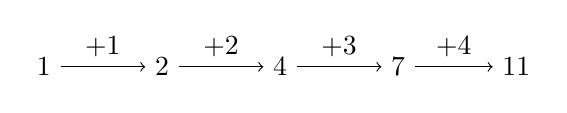
\begin{tikzpicture}
\node (A) at (0,0) {$1$};    
\node (B) at (1.5,0) {$2$};
\node (C) at (3,0) {$4$};
\node (D) at (4.5,0) {$7$};
\node (E) at (6,0) {$11$};

\draw[->] (A) -- (B) node[midway, above] {$+1$};
\draw[->] (B) -- (C) node[midway, above] {$+2$};
\draw[->] (C) -- (D) node[midway, above] {$+3$};
\draw[->] (D) -- (E) node[midway, above] {$+4$};
\end{tikzpicture}
\end{center}
\end{itemize}
\end{example}
\begin{remark}
Une suite arithmétique est constante (tous ses termes sont égaux) si et seulement si sa raison est égale à $0$.
\end{remark}
\begin{proposition}
Soit $\left(u_n\right)_{n \in \N}$ une suite arithmétique de raison $r$. Alors, son $n$\ieme{} terme est donné par la formule
\begin{equation*}
u_0 + n \times r
\end{equation*}
\end{proposition}
\begin{example}
\hfill
\begin{enumerate}[label=\emph{\alph*)}]
\item Donner le $5$\ieme{} terme de la suite arithmétique de premier terme $3,5$ et de raison $3$ : \answerline
\item Donner le $10$\ieme{} terme de la suite arithmétique de premier terme $12$ et de raison $-5$ : \answerline 
\end{enumerate}
\end{example}
\begin{tcolorbox}
En résumé, il y a deux types d'écriture pour le $n$\ieme terme d'une suite arithmétique :
\begin{itemize}
\item La formule de récurrence $u_n = u_{n - 1} + r$. Pour vérifier qu'une suite est arithmétique, on vérifie qu'on obtient chaque terme en ajoutant $r$ au terme précédent.
\item La formule explicite $u_n = u_0 + n \times r$. On l'utilise une fois qu'on sait qu'une suite est arithmétique, pour calculer directement le $n$\ieme{} terme.
\end{itemize} 
\end{tcolorbox}
\newpage
\section{Étude d'une suite arithmétique}
\subsection{Variation d'une suite arithmétique}
\begin{proposition}
\hfill
\begin{itemize}
\item Une suite arithmétique de raison $r$ est \textbf{croissante} si et seulement si $r$ est positive.
\item Une suite arithmétique de raison $r$ est \textbf{décroissante} si et seulement si $r$ est négative.
\end{itemize}
\end{proposition}
\begin{example}
La suite arithmétique
\begin{equation*}
2; 5; 8; 11; \dots 
\end{equation*}
est \answerline~car sa raison vaut~\answerline.

La suite arithmétique
\begin{equation*}
4; -2; -8; \dots 
\end{equation*}
est \answerline~car sa raison vaut~ \answerline.
\end{example}
\subsection{Représentation graphique}
\begin{proposition}
Soit $(u_n)_{n \in \N}$ une suite arithmétique de raison $n$. Alors les points $(0,u_0)$, $(1,u_1)$, $(2,u_2)$, \dots sont alignés.
\end{proposition}
\begin{example}
\hfill
\begin{center}
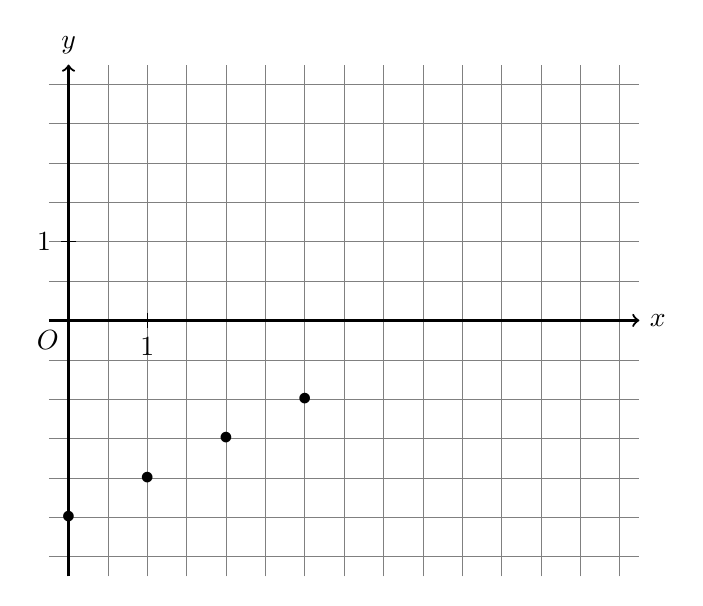
\begin{tikzpicture}
\draw[help lines] (-0.25,-3.25) grid[step=0.5] (7.25,3.25);
\draw[thick,->] (0,-3.25) -- (0,3.25) node[above] {$y$};
\draw[thick,->] (-0.25,0) -- (7.25,0) node[right] {$x$};
\draw (0,0) node[below left] {$O$};
\draw (1,0.1) -- (1,-0.1) node[below] {$1$};
\draw (0.1,1) -- (-0.1,1) node[left] {$1$};

\draw (0,-2.5) node {$\bullet$};
\draw (1,-2) node {$\bullet$};
\draw (2,-1.5) node {$\bullet$};
\draw (3,-1) node {$\bullet$};
\end{tikzpicture}
\end{center}
On a représenté ici les premiers termes d'une suite arithmétique $(u_n)_{n \in \N}$.
\begin{enumerate}[label=\emph{\alph*)}]
\item Quel est le premier terme $u_0$ de cette suite ? \answerline
\item Quelle est la raison $r$ de cette suite ? \answerline
\item Placer les points correspondants aux termes suivants de cette suite.
\item À partir de quel terme (quel $n$ ?) la suite devient positive ? \answerline
\end{enumerate}
\end{example}
\begin{tcolorbox}
\begin{remark}
Un phénoméne représenté par une suite arithmétique suit une évolution dite \textbf{linéaire}.        
\end{remark}
\end{tcolorbox}
\newpage
\section{Moyenne arithmétique}
\begin{definition}
La moyenne arithmétique entre deux nombres $a$ et $b$ est donnée par
\end{definition}
\begin{equation*}
\dfrac{a + b}{2}
\end{equation*}
\begin{example}
Calculer la moyenne arithmétique des couples de nombres suivants :
\begin{enumerate}[label=\emph{\alph*)}]
\item $10$ et $12$ : \answerline
\item $-4$ et $8$ : \answerline
\item $0$ et $0,5$ : \answerline
\item $1,3$ et $1,7$ : \answerline
\end{enumerate}
\end{example}
\begin{proposition}
Soit une suite arithmétique $(u_n)_{n \in \N}$. Alors chaque terme $u_n$ est la moyenne arithmétique du terme précédent et du terme suivant.
\begin{equation*}
u_n = \dfrac{u_{n-1} + u_{n+1}}{2}
\end{equation*}    
\end{proposition}
\vspace{5cm}
\newpage
\section{Somme des premiers termes d'une suite arithmétique}
\begin{definition}
Soit $(u_n)_{n \in \N}$ une suite. Pour parler de la somme $u_0 + u_1 + u_2 + \dots + u_N$, on utilise la notation suivante :
\begin{equation*}
\sum_{n=0}^{N} u_n
\end{equation*}
\end{definition}
\begin{proposition}
Soit $(u_n)_{n \in \N}$ une suite arithmétique, et $N$ un nombre entier. Alors,
$\sum_{n=0}^{N} u_n = (N + 1) \dfrac{u_0 + u_N}{2}$.
\end{proposition}
\begin{remark}
En français, cette formule donnerait
\begin{equation*}
(\text{Nombre de termes à ajouter}) \times \dfrac{\text{Premier terme} + \text{Dernier terme}}{2}
\end{equation*}
\end{remark}
\begin{example}
Calculer les sommes suivantes:
\begin{enumerate}[label=\emph{\alph*)}]
\item $u_0 + u_1 + \dots + u_5$ pour $(u_n)_{n \in \N}$ de premier terme $6$ et de raison $5$.
\item $\sum_{n = 0}^{10} v_n$ pour $(v_n)_{n \in \N}$ une suite arithmétique de premier terme $27$ et de raison $-3$.
\item $\sum_{n = 0}^{42} w_n$ pour $(v_n)_{n \in \N}$ une suite arithmétique de premier terme $15$ et de raison $10$.
\end{enumerate}
\vspace*{8cm} 
\end{example}
\end{document}